The line passes through the given points
\begin{align}
\vec{x}_{1}=\myvec{3\\0} \text{ and } \vec{x}_{2}=\myvec{0\\2}
\end{align}

Since
\begin{align}
\vec{n}^{T}\vec{x}&=1,
\\
\vec{n}^{T}\myvec{3\\0}&=1\\
\vec{n}^{T}\myvec{0\\2}&=1
\end{align}
%
resulting in the the matrix equation
\begin{align}
\myvec{3 & 0 \\ 0 & 2} \vec{n} = \myvec{1 \\ 1}
\end{align}
%
yielding the augmented matrix
\begin{align}
\myvec{3 &0 & 1\\0 & 2 & 1} 
\end{align}
%
Performing row reduction,
\begin{align}
\myvec{3 &0 & 1\\0 & 2 & 1} 
\\
\xleftrightarrow {R_1\leftarrow \frac{R_1}{3}}\myvec{1 &0 & \frac{1}{3}\\0 & 2 & 1}\\ 
\xleftrightarrow {R_2\leftarrow \frac{R_2}{2}}\myvec{1 &0 & \frac{1}{3}\\0 & 1 & \frac{1}{2}}\\
\label{5/5/eq:line_aug}
\end{align}
%
From \eqref{5/5/eq:line_aug},
\begin{align}
\vec{n} = \frac{1}{6}\myvec{2 \\3}
\end{align}
%
Thus the equation of the desired line is 
\begin{align}
\frac{1}{6}\myvec{2 &3}\vec{x} &= 1
\\
\text{or, } \myvec{2 &3}\vec{x} &= 6
\end{align}
Fig. \ref{5/5/Fig:1} plots the desired line.
\begin{figure}[!ht]
\centering
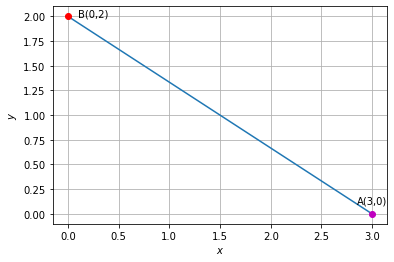
\includegraphics[width=\columnwidth]{image.png}
\caption{Plot obtained from Python code}
\label{5/5/Fig:1}
\end{figure}
